\documentclass[11pt]{article}
\usepackage{geometry}
\usepackage{float}
\usepackage{hyperref}
\usepackage{wrapfig}
\usepackage{bookmark}
\usepackage{comment}
\usepackage{listings}

% Tipografía
\usepackage[sfdefault]{inter}
\usepackage[scaled=0.8]{cascadia-code}
\usepackage{setspace}

%%% BUSCAR SI EXISTE FUENTE HACK


\usepackage{caption}
\captionsetup{%
   labelfont = bf,
   format = plain,
   font = footnotesize
}
\usepackage{biblatex}
\addbibresource{bibliography.bib}

\usepackage{titlesec}

\titleformat*{\section}{\LARGE\bfseries}
\titleformat*{\subsection}{\large}
\titleformat*{\subsubsection}{\large}
\titleformat*{\paragraph}{\large}
\titleformat*{\subparagraph}{\large}

\renewcommand*\contentsname{Resumen de los contenidos}
\renewcommand{\listfigurename}{Tabla de Figuras}

\hyphenpenalty=10000

% Comand para keywords
\providecommand{\keywords}[1]
{
  \small	
  \textbf{\textit{Keywords---}} #1
}

% Setup de hiperenlaces
\hypersetup{
    colorlinks=true,
    linkcolor=cyan,
    filecolor=magenta,      
    urlcolor=cyan,
    pdftitle={deadSet},
    pdfpagemode=FullScreen,
}
 \geometry{
 a4paper,
 total={170mm,257mm},
 left=20mm,
 top=20mm,
 }
 \usepackage{graphicx}
 \usepackage{titling}

 \title{\textbf{\Huge{Videojuego creado en Unity:\\
 \vspace{5mm}
 \textunderscore deadSet}}}
\author{\large{Jesús Jiménez Montero}}
\date{Diciembre 2022}
 
\usepackage{fancyhdr}
\fancypagestyle{plain}{%  the preset of fancyhdr 
    \fancyhf{} % clear all header and footer fields
    \fancyfoot[R]{
\includegraphics[width=2cm]{Images/uanl (1).jpg}}
    %\fancyfoot[L]{\thedate}
    \fancyhead[L]{Videojuego creado en Unity: \textunderscore deadSet}
    \fancyhead[R]{\theauthor}}
\makeatletter
\def\@maketitle{%
  \newpage
  \null
  \vskip 1em%
  \begin{center}%
  \let \footnote \thanks
    {\LARGE \@title \par}%
    \vskip 1em%
    %{\large \@date}%
  \end{center}%
  \par
  \vskip 1em}
\makeatother

%___________________________________________________________
%___________________________________________________________
%___________________________________________________________
%___________________________________________________________
%___________________________________________________________

\begin{document}
\graphicspath{ {./Images/} }
%___________________________________________________________

\vspace{5cm}
\maketitle

\vspace{2cm}

\begin{figure}[H]
    \centering
    
\includegraphics[scale = 1.5]{Images/uanl (1).jpg}
\end{figure}

\vspace{2cm}

\begin{center}
    \begin{tabular}{@{}ll}
        \vspace{1cm}
        \theauthor\\
        \vspace{1cm}
        \large{VJ1202: Informática Básica}\\
        \vspace{1cm}
        \large{Raúl Montoliu Colás}
    \end{tabular}
\end{center}

%___________________________________________________________
%___________________________________________________________
%___________________________________________________________
%___________________________________________________________

\spacing{1.5}

\newpage
\begin{abstract}
    \textunderscore deadSet es un videojuego de acción, estilo twin-stick shooter \cite{twinstickshooters} \footnote{\textit{De Wikipedia: shooter multidireccional en el que el personaje del jugador se controla con dos joysticks: uno para moverse y otro para apuntar y disparar a los enemigos.}} 
    con jugabilidad roguelike \cite{roguelike}. La misión del jugador es sobrevivir el máximo tiempo posible a oleadas de zombis, hasta que llegue la ayuda (la cual es una promesa que nunca llega). Además, el jugador tiene dos armas: un rifle y una escopeta, la cual recarga la munición del rifle. El proyecto consta de la creación de un videojuego creado en Unity, siguiendo las pautas marcadas con el tutorial de Unity dado en clase: “Ruby’s Aventure”. 

    \textunderscore deadSet
    \keywords{Videojuego, Unity, Roguelike}
\end{abstract}
\newpage

\tableofcontents
\newpage

\listoffigures
\newpage

%___________________________________________________________
%___________________________________________________________
%___________________________________________________________
%___________________________________________________________

\section{Propuesta de juego}

    Este juego nació como una idea basada en otro juego. Se modificadron algunas de las ideas y se aplicaron conocimientos de los cuales ya disponía y también nuevos adquiridos durante el curso llevando a desarrollar \textunderscore deadSet. 

    Se quería desarrollar un juego que fuese como la frase en inglés indica: \textit{“easy to learn, hard to master"}\footnote{\textit{Fácil de aprender, difícil de dominar}}; pero que fuese lo más rejugable posible. Por lo tanto, se eligió el género de juego roguelike para esta labor. 

%___________________________________________________________
%___________________________________________________________
%___________________________________________________________
%___________________________________________________________


\begin{comment}
    \section{Herramientas usadas en el proyecto}
    
        Se utilizaron numerosas herramientas para la realización de este juego, las cuales se agruparan por el uso dado:
    
        \subsection{Programación}
            \begin{itemize}
                \item Unity 2020.3.42/43 LTS: Motor de juegos.
                \item Rider 2022.3: IDE con una integración muy elevada con Unity. 
                \item Github (desktop): Gestor .git para gestionar copias del código.
            \end{itemize}
            
        \subsection{Arte}
            \begin{itemize}
                \item Aseprite: Editor de imágenes especializado para pixel-art. 
            \end{itemize}
    
        \subsection{Redacción de documentos}
            \begin{itemize}
                \item Overleaf: Procesador de documentos basado en el lenguaje LaTeX. 
            \end{itemize}
    
\end{comment}

%____________________________________________________________________________________
%____________________________________________________________________________________
%____________________________________________________________________________________
\newpage
\section{Puntos clave del juego y target}
    Los puntos clave de \textunderscore deadSet se pueden resumir en los siguientes: 
    \begin{itemize}
        \item Sistema de combate simple, pero complicado de dominar que balancea el \textit{flow} del juego.
        \item La rejugabilidad es un aspecto importante del juego, haciendo que el jugador quiera mejorar sus tiempos cada vez que quiera volver a jugar para superarse a sí mismo. 
        \item Debido a sus gráficos simples realizados en \textit{pixel-art}, el juego se podrá jugar en una gran cantidad de dispositivos. 
        \item Aunque el juego dispone de mucha rejugabilidad, se pretende ser respetuoso con el tiempo del jugador, con partidas que duran de media entre 10 a 15 minutos, pudiendo ser más si el jugador es muy habilidoso. 
    \end{itemize}
        
        \subsection{Taxonomía de Bartle}
            Otro aspecto crucial del juego es su \textit{target} muy definido. Para lograr esto, se usó la \textit{Taxonomía de jugadores de Bartle} \cite{bartle}, la cual se define como: 
                \begin{itemize}
                    \item \textit{\textbf{Achievers}}: Los cuales prefieren, por ejemplo,  ganar la máxima puntuación en un juego o conseguir todos los logros en un juego. 
                    \item \textit{\textbf{Killers}}: que son los jugadores que prefieren interactuar con otros jugadores y superarlos en algún reto.
                    \item \textit{\textbf{Explorers}}: Que, si tienen un mapa el cual revela el mundo de forma progresiva, preferiran completar el mapa entero y descubrir todos los recovecos que este mundo esconda.
                    \item \textit{\textbf{Socializers}}: Que están dispuestos a relacionarse con la mayor cantidad de jugadores posibles y prefieren el aspecto social de juego. 
                \end{itemize}
    
            \vspace{5mm}
    
            Una vez definida la \textit{Taxonomía de Bartle} \cite{bartle} podemos definir a los potenciales jugadores de \textunderscore deadSet como: 
                \begin{itemize}
                    \item \textit{\textbf{Killers}}: Debido a que el juego se basa principalmente en superar oleadas de enemigos los cuales hay que derrotar usando armas.
                    \item \textit{\textbf{Achievers}}: Debido a la presencia de un temporizador dentro del juego que hará que este tipo de jugadores se quieran superar cada vez que jueguen.
                \end{itemize}

%____________________________________________________________________________________
%____________________________________________________________________________________
%____________________________________________________________________________________

\section{Jugabilidad y Mecánicas}
    \subsection{Modo de juego}
        El juego dispone de un único modo de juego, el cual consiste de oleadas de enemigos, en el que el jugador se enfrenta a ellos generados de forma aleatoria por el mapa, y una vez son derrotados, el juego genera más enemigos dependiendo del número de oleadas.\\

    \subsection{Dinámicas}
        La dinámica más presente del juego es la gestión de munición, ya que el jugador tiene que tener en mente el número de balas restantes; además de que todas las acciones del jugador requieren de un tiempo para realizarse, siendo una de las más duras recargar la escopeta porque se necesita munición de escopeta para recargar el rifle. \\
    
    \subsection{Mecánicas de combate}
        \textunderscore deadSet es un roguelike en el que si el jugador muere, la partida se acaba y el juego se reiniciará desde la oleada 1. Al jugador para defenderse de los zombis se le proporcionan dos armas:
        
            \begin{itemize}
            
                \item \textbf{Rifle de asalto}: Rifle con una alta cadencia de tiro y preciso pero un daño bajo. Versátil y capaz de derrotar varios enemigos con un solo cargador.\\ 
                Aunque, no se puede recargar de forma manual.\\ 
                Como mecánica adicional, el jugador recarga el rifle disparando la escopeta; es decir, cuando el jugador dispara la escopeta, se restaura el cargador del rifle.\\
                
                \item \textbf{Escopeta}: Arma muy potente, capaz de derrotar un enemigo de un solo disparo; aunque lenta de usar. Es el arma primaria del jugador debido a que es muy potente, aunque al contrario del rifle, se necesita recargar la escopeta de forma manual usando un botón.\\ 
                Por motivos de balanceo, el cargador de la escopeta es pequeño y se recarga como una escopeta de bombeo (es decir, cada vez que el jugador dispara tiene que esperar para disparar de nuevo). Además, para recargarla se hace de forma manual cartucho a cartucho (es decir, se introduce una bala en el cargador cada cierto tiempo).\\

            \end{itemize}

        
        Además, cada oleada acabada en 1, activa un método (ver código debajo: \ref{fig:waveacabada1}) para mejorar las armas las cuales mejoran ligeramente las estadísticas de las armas hasta llegar a un umbral concreto. \\ 
        
        \begin{figure}[H]
            \centering
            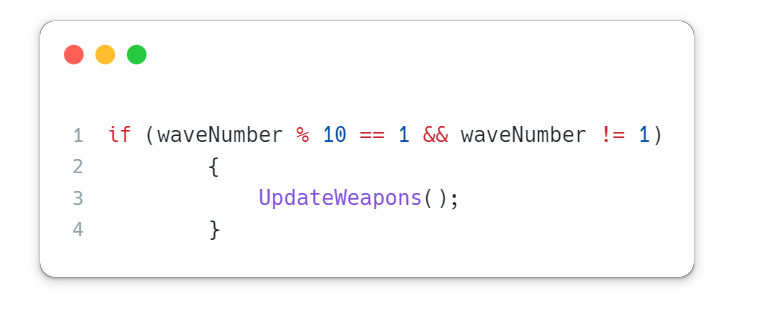
\includegraphics[width=\textwidth]{Images/Menuprincipal/wavnumber.png}
            \caption{Método para mejorar las armas}
            \label{fig:waveacabada1}
        \end{figure}

        Otros aspectos destacables del combate son cuando se daña el personaje o los zombis. Comenzando por los zombis:\\
        
        Cuando una bala lo toca, cambia su color para señalizar que ha sido golpeado, y suavemente vuelve a su color original; esto se hizo para darle más importancia al golpe y resaltar al jugador que ha dañado al enemigo.\\ 

        Esto también ocurre cuando los zombis dañan al jugador. El zombi que ha golpeado al jugador se resalta (esta vez la duración siendo el \textit{cooldown} necesario para volver a hacer daño al jugador).\\
        
        Esto también ocurre con el \textit{sprite} del jugador para resaltar que ha sido dañado. El desvanecimiento del color es el mismo que el \textit{cooldown} de los zombis y puede ser activado tantas veces el jugador se choque contra un zombi.\\

        \newpage
        \subsection{Bucle de juego}
        \textunderscore deadSet se caracteriza por tener un bucle de juego muy definido y cerrado, el cual se puede definir como:
        
        \begin{itemize}
            \item Derrotar oleada de enemigos → Pasar de oleada → Oleada Fuerte → Mejora de Armas → Repetir
        \end{itemize}
        Este de hecho se podría definir como el bucle de juego principal, aunque hay otros bucles aún más cerrados, pero menos obvios al jugador debido a que se integran con este.\\
        
        Estos bucles serían, por ejemplo, el propio hecho de usar las armas. Aunque tampoco se puede considerar un bucle cerrado, ya que las armas se pueden usar en el orden que el jugador quiera. Podemos representarlo como este bucle de ejemplo:\\
        \begin{itemize}
            \item Disparar rifle → Agotar munición → Disparar escopeta → Disparar rifle → Agotar ambas municiones → Recargar escopeta → Repetir
        \end{itemize}
%____________________________________________________________________________________
%____________________________________________________________________________________
%____________________________________________________________________________________
\newpage
\section{Elementos que componen el juego}
    En este apartado se explican los \textit{assets} que componen el juego, los cuales están listados de forma concisa en el \href{https://github.com/JesusJMUJI/TopDownShooterGame}{GitHub del proyecto}. 
    
    \subsection{Interfaz de Usuario}
        Uno de los objetivos que se quería conseguir con el juego era ser minimalista en cuanto al diseño, incluyendo la interfaz.  
        \begin{figure}[H]
            \centering
            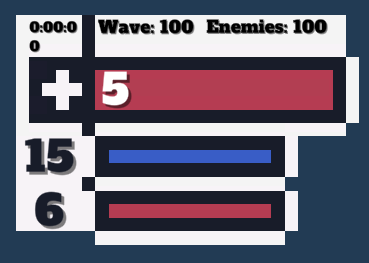
\includegraphics[scale = 0.7]{Images/UI.png}
            \caption{Interfaz del juego}
            \label{fig:UI}
        \end{figure}
        
        Se usaron elementos minimalistas para generar la interfaz del juego, con un aspecto de bloques y números con una fuente lo más legible posible. Con las barras de munición (azul y rojo para el rifle y la escopeta, respectivamente) agotándose según las balas restantes en el cargador, además del número mencionado para los jugadores que prefieran saber exactamente cuanta munición les queda.\\
        
        Se probó otra variante de los contadores, incluyéndolos al lado del arma. Aunque se descartó la idea debido a que los contadores eran demasiado pequeños y podían dar lugar a confusión al leerlos.\\
        
        \begin{figure}[H]
            \centering
            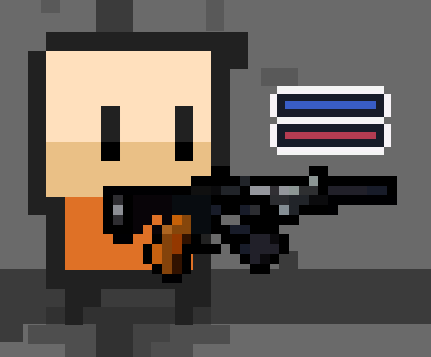
\includegraphics[scale = 0.5]{Images/UI descartada.png}
            \caption{Interfaz al lado del arma}
            \label{fig:UI descartada}
        \end{figure}
        
    \subsection{Elementos gráficos}
        
        Para simplificar el proceso de desarrollo del juego, se utilizaron \textit{assets} comprados con licencia de uso personal/comercial, los cuales se pueden encontrar en el \href{https://github.com/JesusJMUJI/TopDownShooterGame}{GitHub del proyecto}.\\
        
        Un resumen del uso de los \textit{assets} gráficos sería:
        \begin{itemize}
            \item \textbf{2D Top Down Shooter Game Assets}: Starter Kit, para el \textit{tileset}, los personajes y la cruceta.
            \item \textbf{Tech Dungeon: Roguelite}: para interfaz del juego, \textit{(Demo del paquete)}
            \item \textbf{Pixel Art Guns Pack + Animations}: Para las armas con sus respectivas animaciones, además de las balas.
        \end{itemize}
        
        Aún habiendo usado \textit{assets} comprados, se quiso dar un toque personal al juego, creando el logotipo a mano. Para esta labor, se usó el software gráfico Aseprite \cite{aseprite}, dando este resultado:
        \begin{figure}[H]
            \centering
            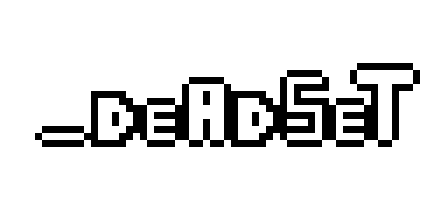
\includegraphics[width=\textwidth]{Images/logo_big.png}
            \caption{Logotipo del juego}
        \end{figure}
        
        Para futuros proyectos, un objetivo a alcanzar sería poder realizar todos los \textit{assets} gráficos a mano.
    
    \subsection{Apartado sonoro}
        
        Para el sonido del juego, se tenía un objetivo en mente, el cual es: \textit{“punchy”}, traducido al castellano como “impactante”. Se buscaban sonidos que fuesen poco monótonos, ya que el juego se basa en disparar todo el tiempo, así que no se podían usar sonidos que fuesen genéricos o “aburridos”.\\

        Además, un problema que al jugador se le presenta es quedarse sin munición. Se quería que el jugador siempre tuviese presente su número de balas restante y para indicar que su cargador se había agotado, se añadió un \textit{click} cuando intentas disparar y no te queda munición.\\
        
        % AÑADIR ENLACE AL PAQUETE DE SNAKE
        Se usaron los sonidos del paquete \textit{Snake's Authentic Gun Sounds(1 y 2)}.\\
        
        Aparte de los sonidos de \textit{Snake}, se usó para sonido de la escopeta un sonido de una librería C00: Sonniss.com - GDC 2016 - Game Audio Bundle / TS Sound → 12 Gauge Shotgun.\\
        
        Para la \textit{OST} se necesitaba música que no hiciese monótonas las partidas. Ya que, un juego que esté diseñado para ser rejugable necesita precisamente romper esta monotonía. Un ejemplo para resolver esta situación es que cada vez una canción acaba, el \textit{script} \textit{Sound\textit{Script}} [\ref{fig:musica}] de forma aleatoria una canción de una lista de canciones.\\
        
        % AÑADIR ENLANCE AL ACTION MUSIC PACK
        Para estas canciones se usó la música de \textit{Action Music Pack 1 y 2}.\\
        
    \subsection{Otros elementos}
    
        % AÑADIR ENLACE A LA FUENTE EN GOOGLE FONTS
        Comentando otros \textit{assets} usados en el juego, para el menú principal se usaron \textit{\textit{sprite}s} del paquete: \textit{Controller \& Keyboard Icons}, ya que se querían representar los controles de una manera más “táctil”, visual o intuitiva.\\
        
        En cuanto a la fuente se buscaba una fuente que fuese más desenfadada y fuese fácil de leer en un “momento de pánico”. Por lo que se escogió la fuente: Alfa-Slab One, la cual está disponible en \textit{Google Fonts} de forma gratuita y de uso libre.\\

\newpage
\section{¿Cómo se ha creado el juego?}
    En esta sección se explicará como se han creado algunos de los puntos más importantes del juego, destacando \textit{scripts} importantes.
    \subsection{Menú principal}
        El juego, debido a su complejidad mecánica y numerosos controles, se quería implementar de alguna manera una forma sencilla de comprender los controles y una guía de juego dentro de este mismo.\\

        Para esto, se crearon tres \textit{Paneles de UI}, los cuales permiten meter varios elementos de interfaz juntos.\\
        \begin{figure}[H]
            \centering
            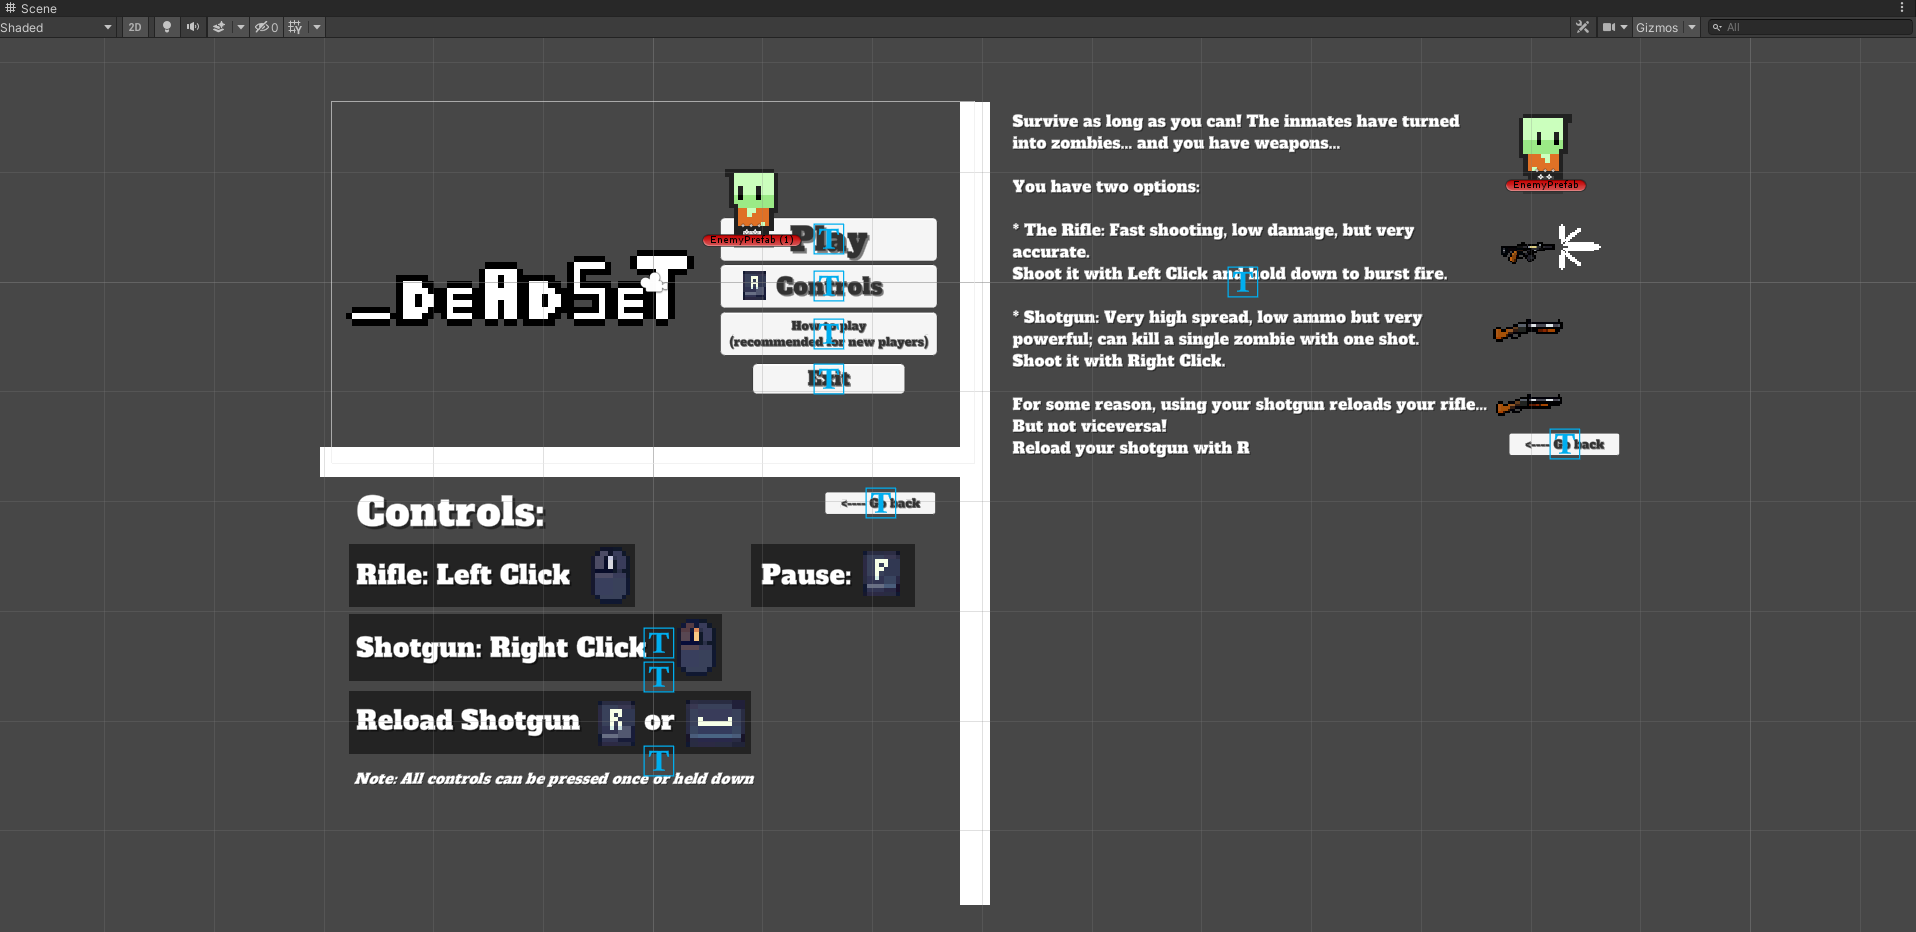
\includegraphics[width=\textwidth]{Images/Menuprincipal/Paneles.png}
            \caption{Paneles de UI}
        \end{figure}

        Y para que la cámara se moviese a esos paneles, se crearon varios objetos vacíos, los cuales se usan en el código a modo de referencia para poder mover la cámara al lugar concreto. \\
        Cuando presionas un botón (\textit{excepto el botón Play}) con un método el cual acepta un valor \texttt{Vector3 target}, coge el \textit{transform} del objeto vacío y activa una corrutina que interpola el movimiento hasta llegar a la posición del objeto vacío. \\
        \begin{figure}[H]
            \centering
            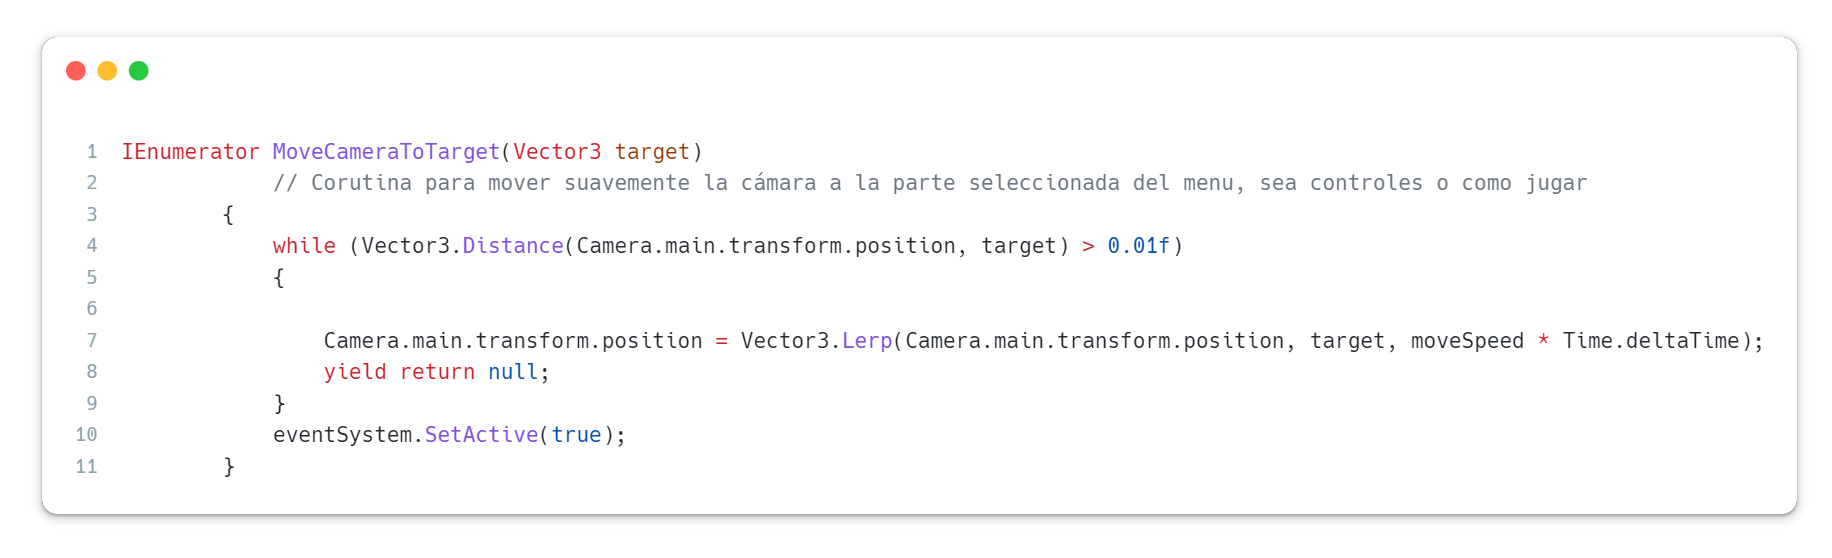
\includegraphics[width=\textwidth]{Images/Menuprincipal/corutinacamara.png}
            \caption{Corrutina para mover cámara al \textit{target}}
        \end{figure}

    \newpage
    \subsection{Enemigos} \label{fig:enemigos}
        Una parte importante de los enemigos es que tienes que derrotarlos porque no vale solo con esquivarlos. Era primordial saber si la bala ha impactado correctamente. \\
        Para esto, se hizo una función que hace que el enemigo cambie de color cuando le has golpeado y después de forma suave cambie de nuevo a su color original. \\
        \begin{figure}[H]
            \centering
            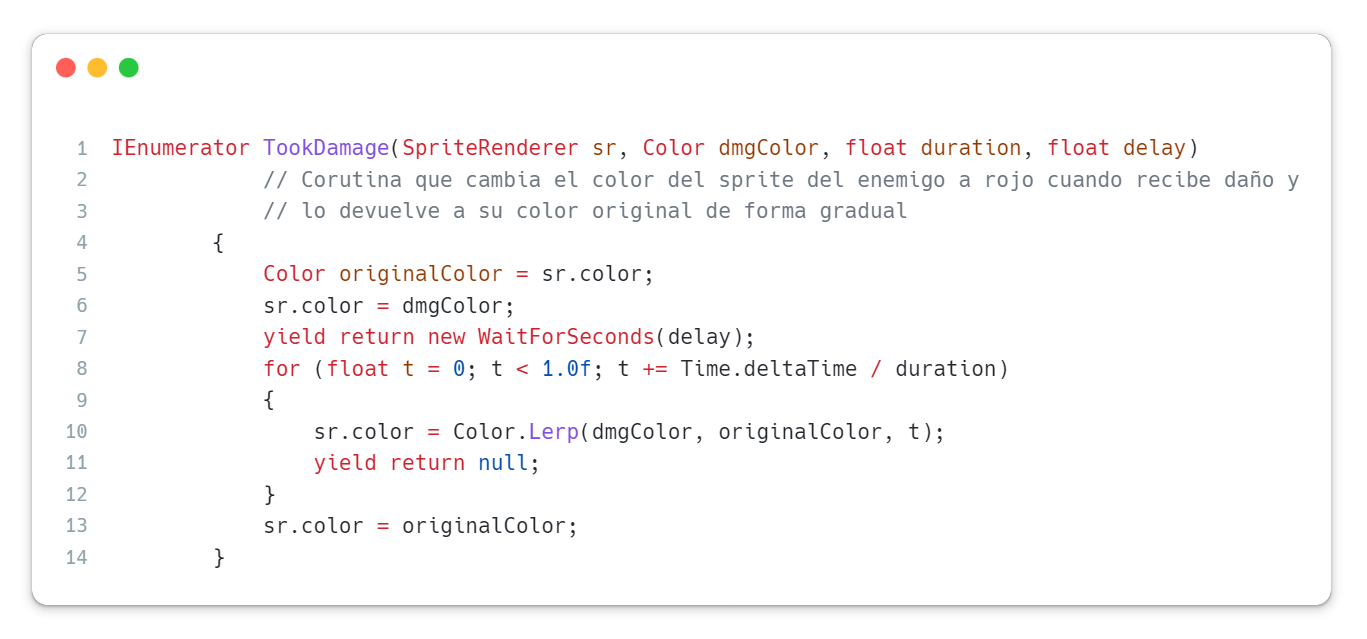
\includegraphics[width=\textwidth]{Images/Menuprincipal/TookDamage.png}
            \caption{Corrutina para cambiar de color al dañar el enemigo}
        \end{figure}
        Esta corrutina acepta unos parámetros concretos, lo cual ayuda a la hora de programar estos cambios.\\

        También se usa \textit{desvanecimiento} para cuando los enemigos aparecen en una nueva oleada para hacer un poco más amena la introducción de nuevos enemigos en el mapa.
        \begin{figure}[H]
            \centering
            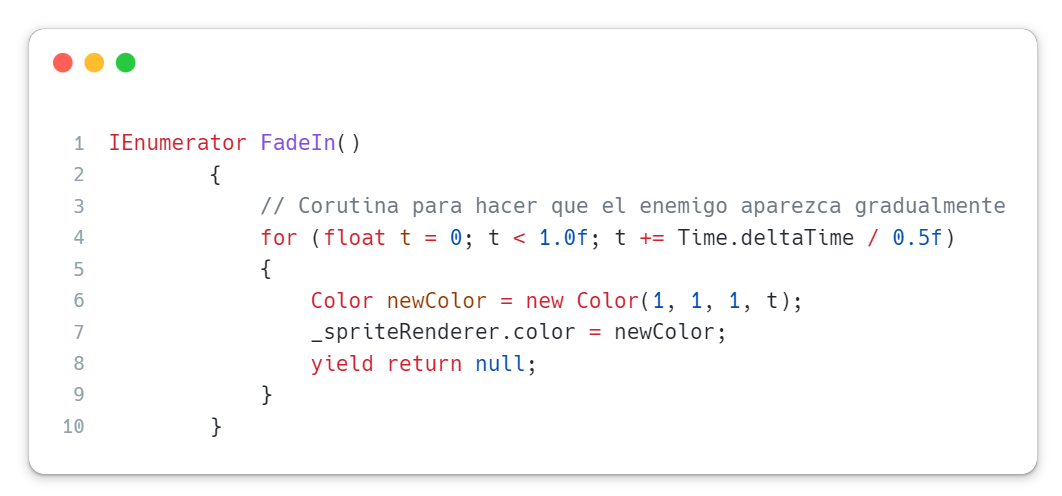
\includegraphics[width=\textwidth]{Images/Menuprincipal/fadein.png}
            \caption{Corrutina para hacer desvanecer al enemigo}
        \end{figure}
    \subsection{Jugador}

    \begin{wrapfigure}{r}{0.2\textwidth}
        \begin{center}
            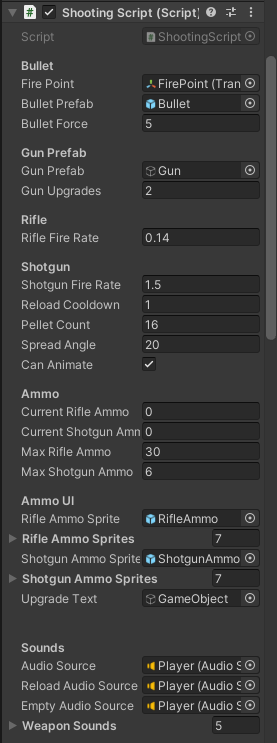
\includegraphics[width=0.2\textwidth]{Images/ShootyMacShooty/rifleinspector.png}
            \caption*{Inpector del \textit{script} \textit{Shooting \textit{script}}}
        \end{center}
        \caption{Player}
    
    \end{wrapfigure}        

        Desde el punto de vista del jugador, una parte muy importante es todo lo relacionado con disparar, lo que se controla desde un \textit{script} que sirve para exclusivamente esto. Principalmente, el \textit{script} se divide en diferentes partes:

        \begin{itemize}
            \item Rifle 
            \item Escopeta
            \item Función de recarga de la escopeta
        \end{itemize}
        Se explicará a continuación cada una de estas partes.\\
        \newpage

        \subsubsection{Rifle} \label{rifle}
            Una parte del \textit{script} se encarga de la lógica del rifle, la cual es más sencilla que la escopeta.

            En primer lugar se ejecuta la parte del \textit{disparo}, la cual instancia una bala junto a una variable de fuerza y según donde esté apuntando la mira (\textit{crosshair en inglés}).\\

            Después se inicia otro método que se encarga de actualizar el \textit{sprite} de la barra de munición.\\ 
            La cual actualiza / refresca el \textit{sprite} cada vez que el contador de munición sea múltiplo de 5: \texttt{int index = (currentRifleAmmo / 5) - 1;}. \\

            Ambos pasos ocurren en ambos \textit{scripts}, aunque la escopeta tiene variaciones que explican en la sección~\ref{escopeta}.

            \begin{figure}[H]
                \centering
                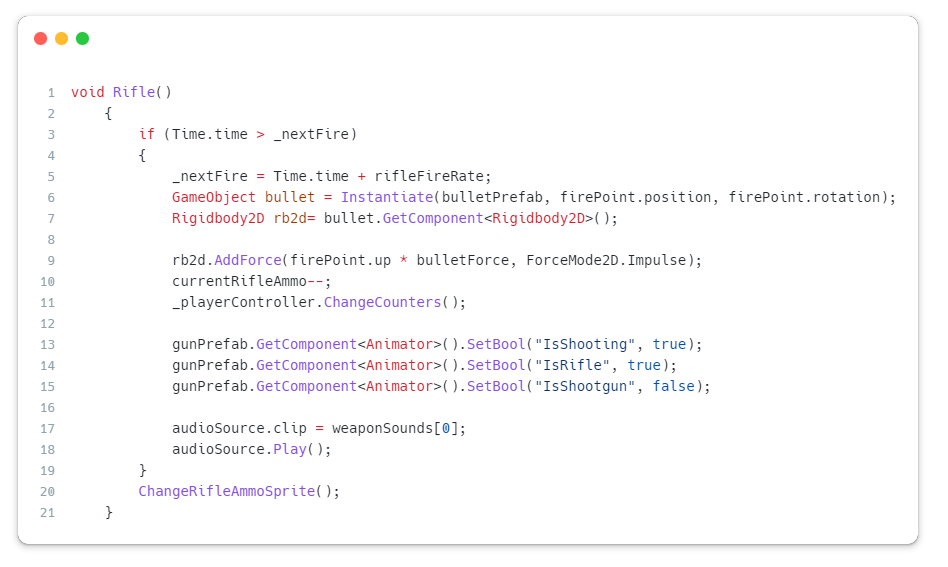
\includegraphics[width=\textwidth]{Images/ShootyMacShooty/rilfe.png}
                \caption{Parte del \textit{script} que se encarga del rifle}
            \end{figure}
        \newpage
        \subsubsection{Escopeta} \label{escopeta}
            La escopeta varía con el rifle en que tiene que generar varias balas / proyectiles / perdigones.\\

            Para esto, en el \texttt{void Awake()} se inicializa una lista de \textit{Quaternions} creados con un bucle, según cuantas balas se hayan asignado.\\ 

            Y cuando el jugador dispara ocurre esto:\\
            \begin{figure}[H]
                \centering
                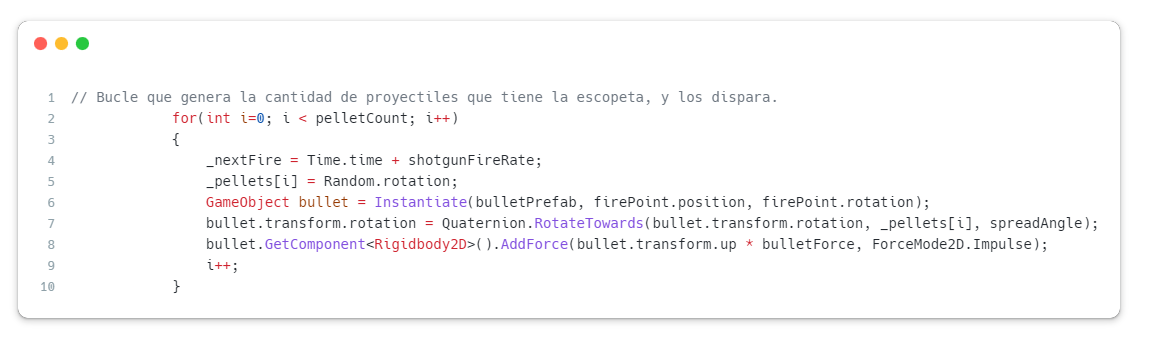
\includegraphics[width=\textwidth]{Images/ShootyMacShooty/shootpelletes.png}
                \caption{Bucle para disparar las balas de la escopeta}
            \end{figure}
            Parece una función algo enrevesada, pero, resumiéndola brevemente:
            \begin{enumerate}
                \item Se reinicia el \textit{cooldown} para poder disparar y se reinicia este mismo.
                \item Se recorre la lista, asignando el valor \texttt{Random.rotation} a los \textit{Quaterniones} de la lista.
                \item Se instancia la bala igual que en el rifle (sección:~\ref{rifle})
                \item Se aplica \textit{spread}[\footnote{traducido como propagación}]para crear aleatoriamente la dirección de los proyectiles. 
                \item Y por último, se le aplica la fuerza a la bala.
            \end{enumerate}
            También se ejecutan las instrucciones de refrescar la barra de munición, pero cada vez que disparas la escopeta debido al bajo cargador de munición del que dispone (no como en el rifle que es cada múltiplo de cinco). \\
            
        \newpage
        \subsubsection{Función de recarga de la escopeta}  
            Método muy sencillo en el que añade una bala al cargador de la escopeta, según el valor de la variable \texttt{currentShotgunAmmo} no sea inferior o superior a valor máximo de \texttt{currentShotgunAmmo}.\\
            También se comprueba si se puede recargar con la variable \texttt{canAnimate}, que se usa para que no puedan solaparse las animaciones de la escopeta. 
            \begin{figure}[H]
                \centering
                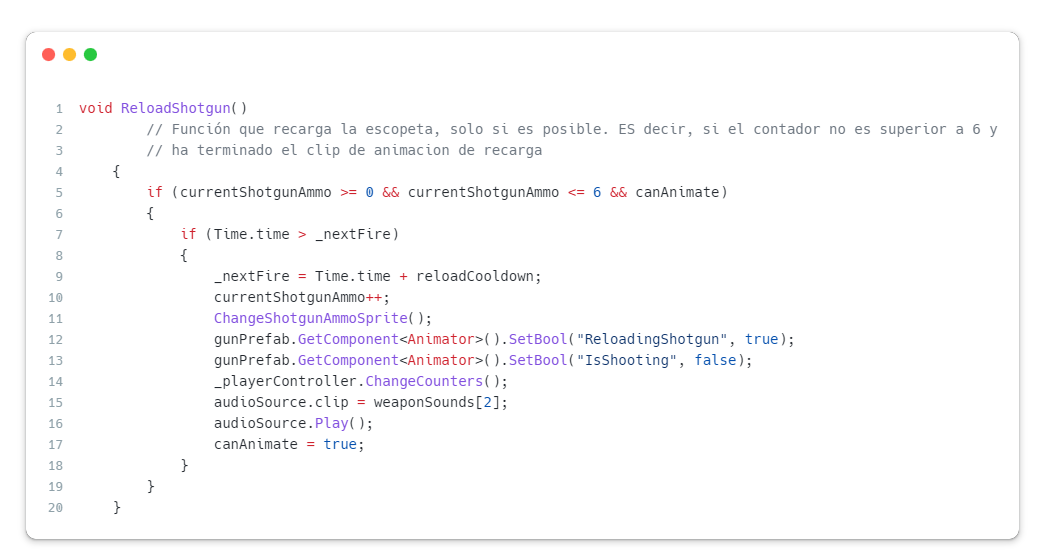
\includegraphics[width=\textwidth]{Images/ShootyMacShooty/reload.png}
                \caption{Función de recarga de la escopeta}
            \end{figure}
    \newpage
    \subsection{Funciones Específicas}
        En esta sección se explican otros \textit{script}s que se encargan de funciones más específicas. Son las siguientes:\\
        \begin{itemize}
            \item \textit{Crosshair}[\footnote{También conocido como mira, mirilla o cruceta. Es el cursor que se usa para apuntar.}]
            \item Gestor de oleadas
            \item Contador de Enemigos
            \item Generador de posiciones aleatorias
            \item Generador de oleadas de enemigos
            \item Balas
            \item Pivote de arma
            \item Gestor de música
        \end{itemize}

        \subsubsection{\textit{Crosshair}}
            Como el videojuego es un juego de disparos top-down, se necesitaba una forma de apuntar a los enemigos  que no fuese de forma direccional, como en Ruby's Adventure. Se decidió usar el método de los roguelikes topdown modernos, usando un cursor que se mueva con el ratón, y que se actualice según la posición del jugador.\\
            \begin{figure}[H]
                \centering
                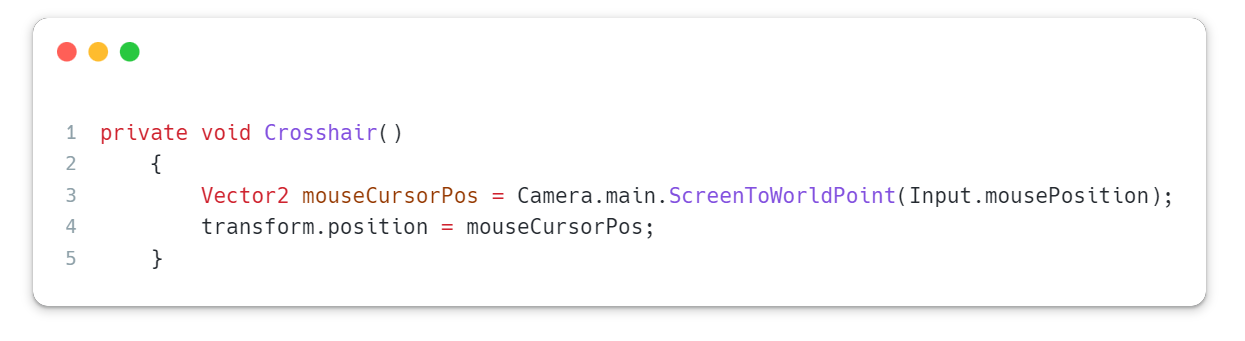
\includegraphics[width=\textwidth]{Images/Misc/crosshair.png}
                \caption{\textit{Script} para actualizar la posición de la mirilla}
            \end{figure}
        
        \newpage
        \subsubsection{Gestor de oleadas}
            Para la labor de controlar el aspecto de las oleadas de enemigos, se usa un \textit{script} llamado \textit{GameManager}, el cual se ocupa de funciones más globales que no se pueden encargar en otros \textit{script}s más individuales.\\
            \begin{figure}[H]
                \centering
                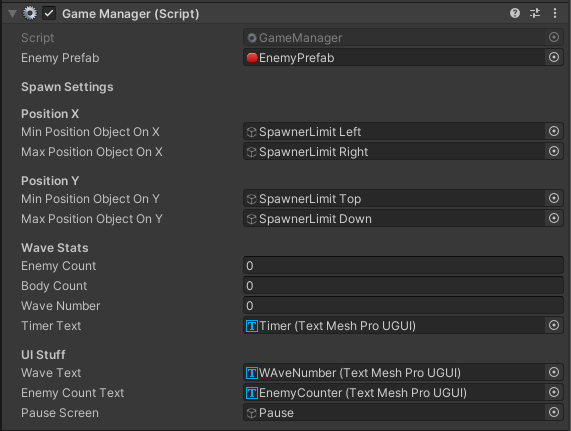
\includegraphics[width=0.7\textwidth]{Images/Misc/inspectorgamemanager.png}
                \caption{GameObject vacíos referenciados en el inspector del \textit{script} \texttt{GameManager}}
                \label{fig:inspectorgamemanager}
            \end{figure}

            \newpage
            \subsubsection{Contador de Enemigos}
                Este \textit{script} se encarga de controlar el número de enemigos que quedan en la oleada, y de generar la siguiente oleada de enemigos.\\
                \begin{figure}[H]
                    \centering
                    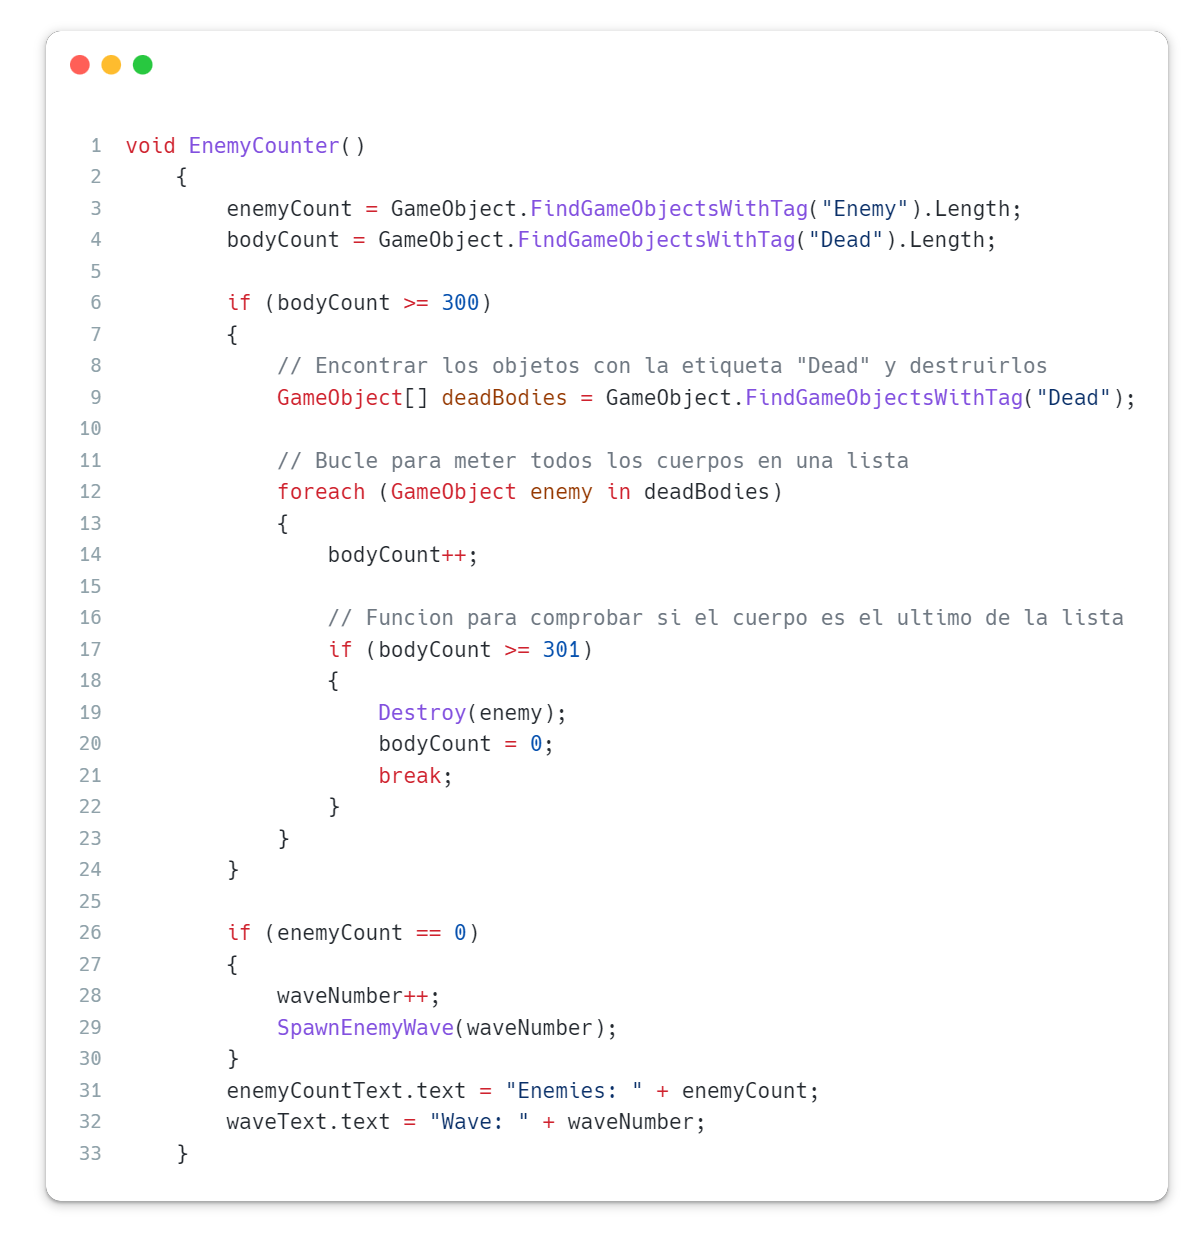
\includegraphics[width=\textwidth]{Images/Misc/EnemyCounter.png}
                    \caption{\textit{Script} para controlar el número de enemigos que quedan en la oleada}
                \end{figure}

                \newpage
                La primera parte de la función de este \textit{script} es bastante simple, esta comprueba el número de enemigos cada vez que un enemigo muere.\\ 
                
                Sin embargo, a continuación se revela su potencial, debido a que comprueba dos tipos de enemigos, los vivos y los muertos (debido a que cuando un enemigo muere, en su código cambia su \textit{tag} a \texttt{"Dead"}).\\

                Aunque una parte destacable del \textit{script} es la parte de \texttt{bodyCount}. Cuando el conteo de "cuerpos" sea 301, se inicializa una función que añade todos los cuerpos a una lista (de GameObjects) y recorre esta lista y si mide más de 301, se destruye el GameObject 301.\\

                Se hace esto para evitar que el juego se ralentice debido a que hay demasiados GameObjects en la escena además de para no saturar de cuerpos el terreno de juego.\\

            \newpage
            \subsubsection{Generador de posiciones aleatorias}
                \begin{figure}[H]
                    \centering
                    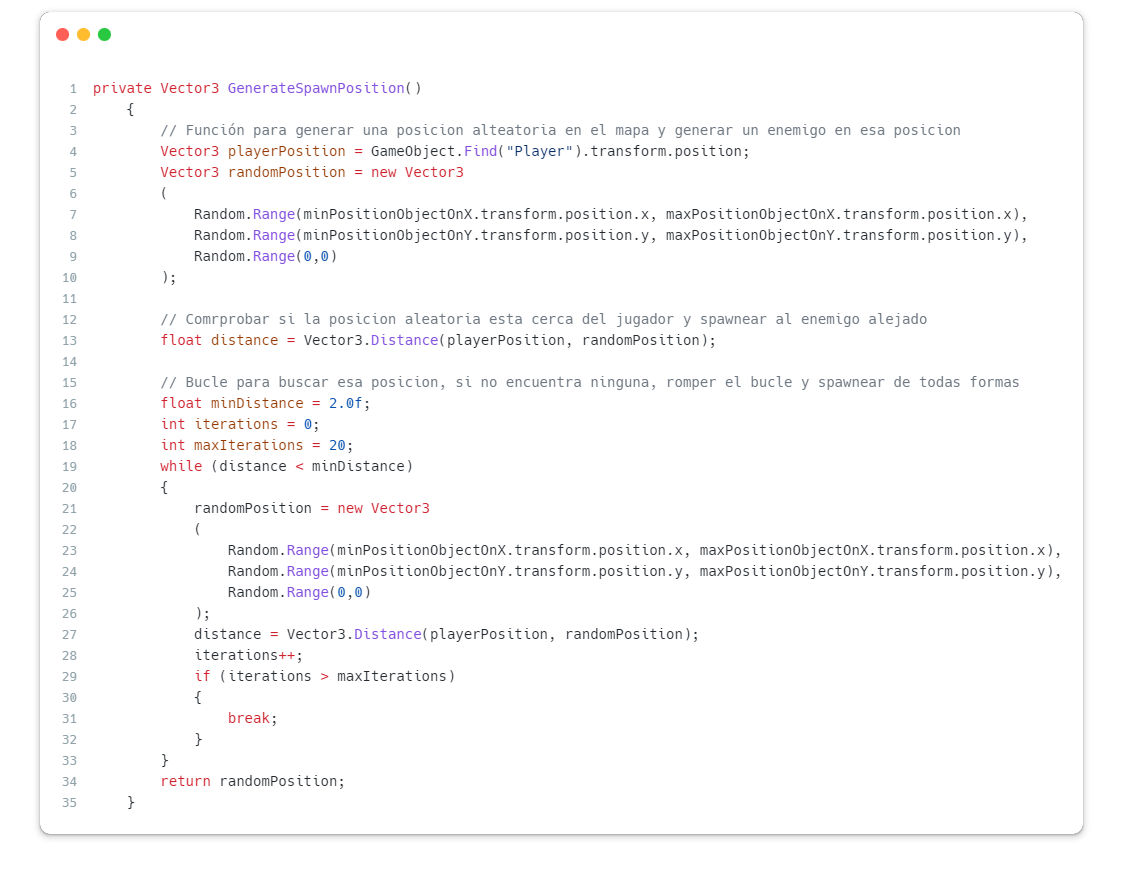
\includegraphics[width=\textwidth]{Images/Misc/generatespawnposition.png}
                    \caption{\textit{script} para generar posiciones aleatorias}
                \end{figure}
                La función de generar una posición es bastante compleja, ya que se encarga de generar una posición aleatoria en el mapa y la zona de \textit{spawn} no este cerca jugador en todo lo posible.\\

                Primero, se crearon 4 objetos vacíos (llamados \textit{SpawnerLimits}), uno para cada lado del mapa. En la figura~\ref{fig:inspectorgamemanager} se puede ver como se han referenciado en el inspector del \textit{script}.\\

                Cuando una oleada necesita ser generada, se crea una \texttt{randomPosition} como \texttt{Vector3}, cuyos componentes x,y,z tienen un \texttt{Random.Range} entre los límites mínimos y máximos de X e Y, dados por el componente \texttt{Transform} de los \texttt{GameObject} vacíos referenciados.\\
                \begin{figure}[H]
                    \centering
                    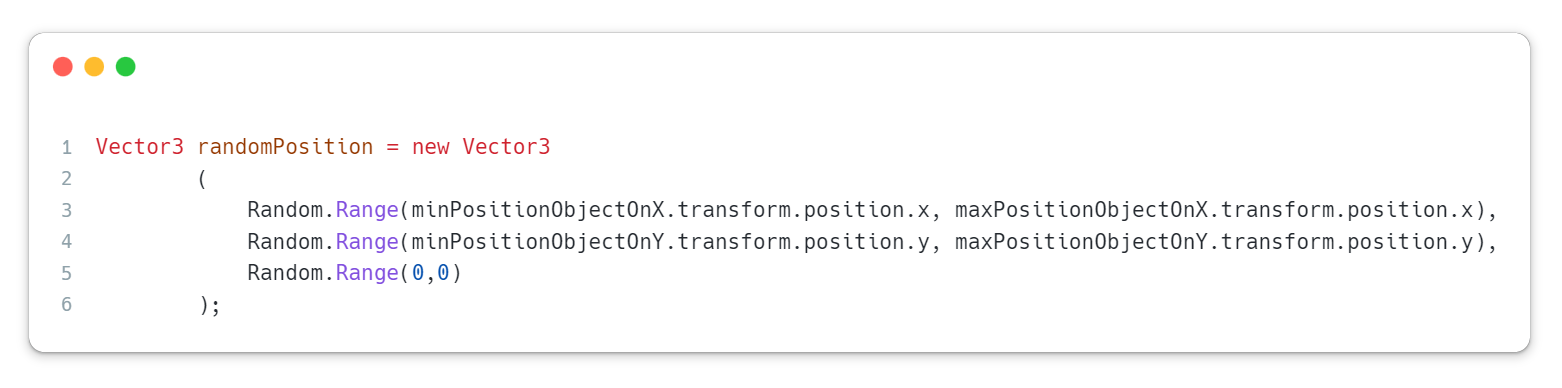
\includegraphics[width=\textwidth]{Images/Misc/randompos.png}
                    \caption{Generación de una posición aleatoria}
                    \label{fig:randompos}
                \end{figure}

                Aunque esto no es suficiente, ya que si se genera una posición aleatoria, puede que la posición sea muy cercana al jugador y lleve a situaciones injustas como recibir daño que sería imposible de esquivar, por lo que se necesita una segunda comprobación.\\
                \begin{figure}[H] 
                    \centering
                    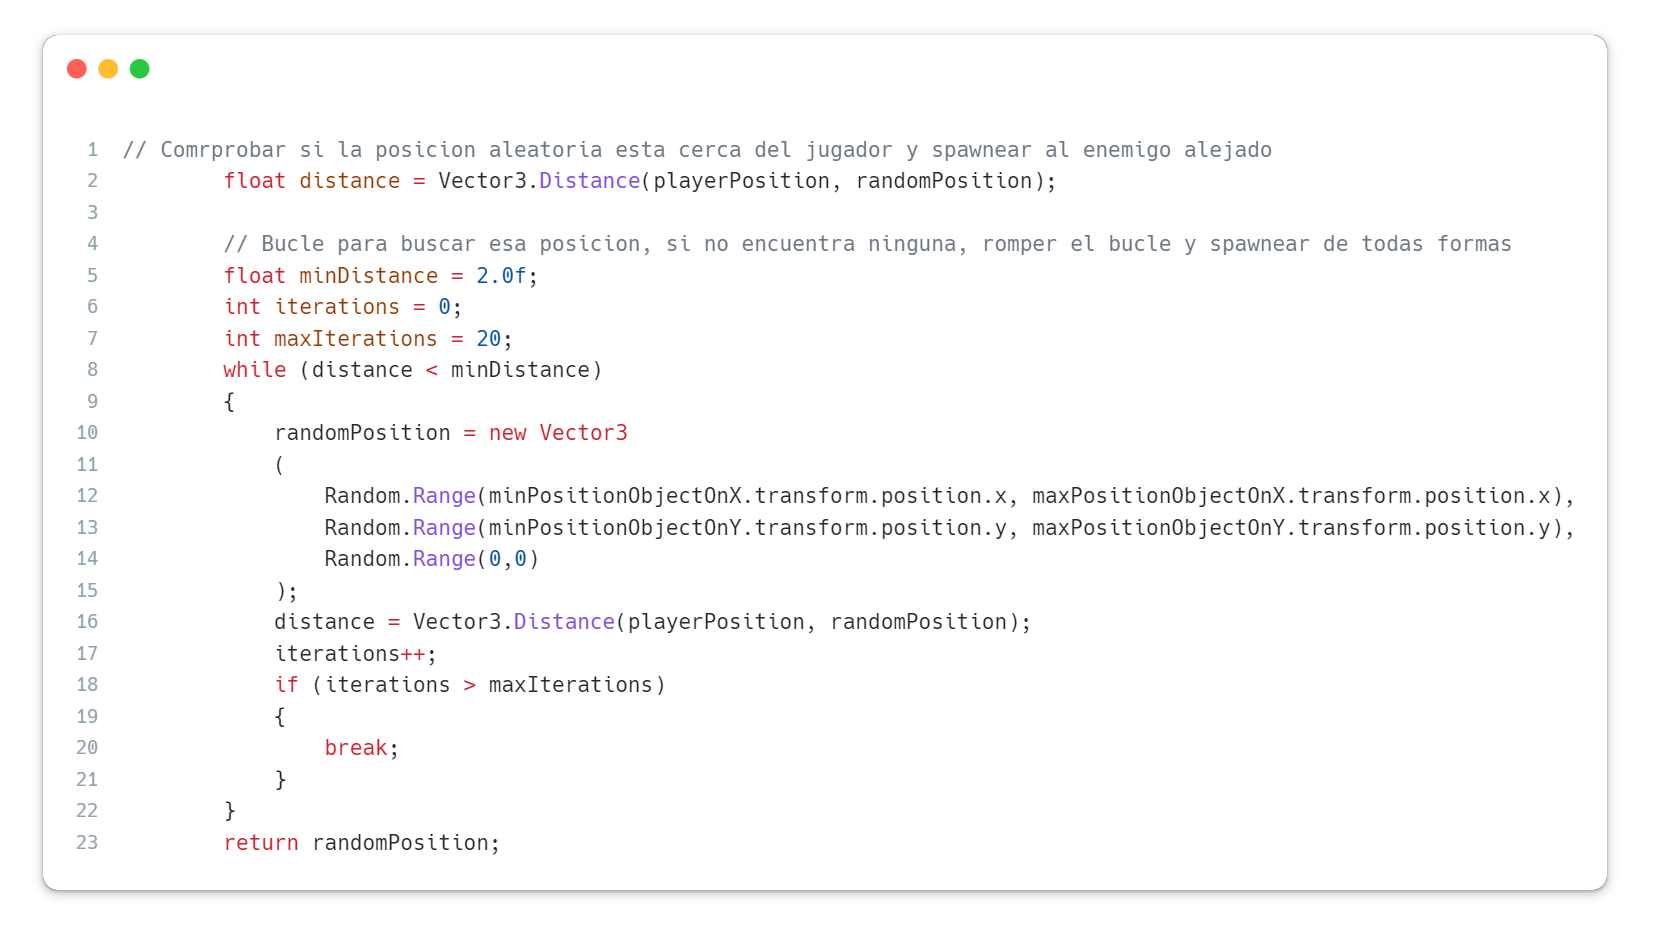
\includegraphics[width=\textwidth]{Images/Misc/comprobacionspawn.png}
                    \caption{Comprobación de la distancia entre la posición aleatoria y el jugador}
                \end{figure}
                Lo que hace esta función es delimitar una distancia de un \texttt{Vector3} comprendido entre la posición del jugador y la posición generada del enemigo en la función anterior (ver figura \ref{fig:randompos}).\\ 

                \newpage
                Y se comprueba con un bucle que la distancia sea menor a la distancia mínima para generar a los enemigos.\\

                Además, para que este bucle no sea infinito y Unity se detenga, hay un máximo número de iteraciones que el generador tiene disponible, y si llega a este número, se rompe el bucle y se genera al enemigo independientemente de que vaya a reaparecer cerca del jugador. Esto es más notable en oleadas con muchos enemigos (rondas con más de 100 enemigos).\\

            \newpage
            \subsubsection{Generador de oleadas de enemigos}
                \begin{figure}[H]
                    \centering
                    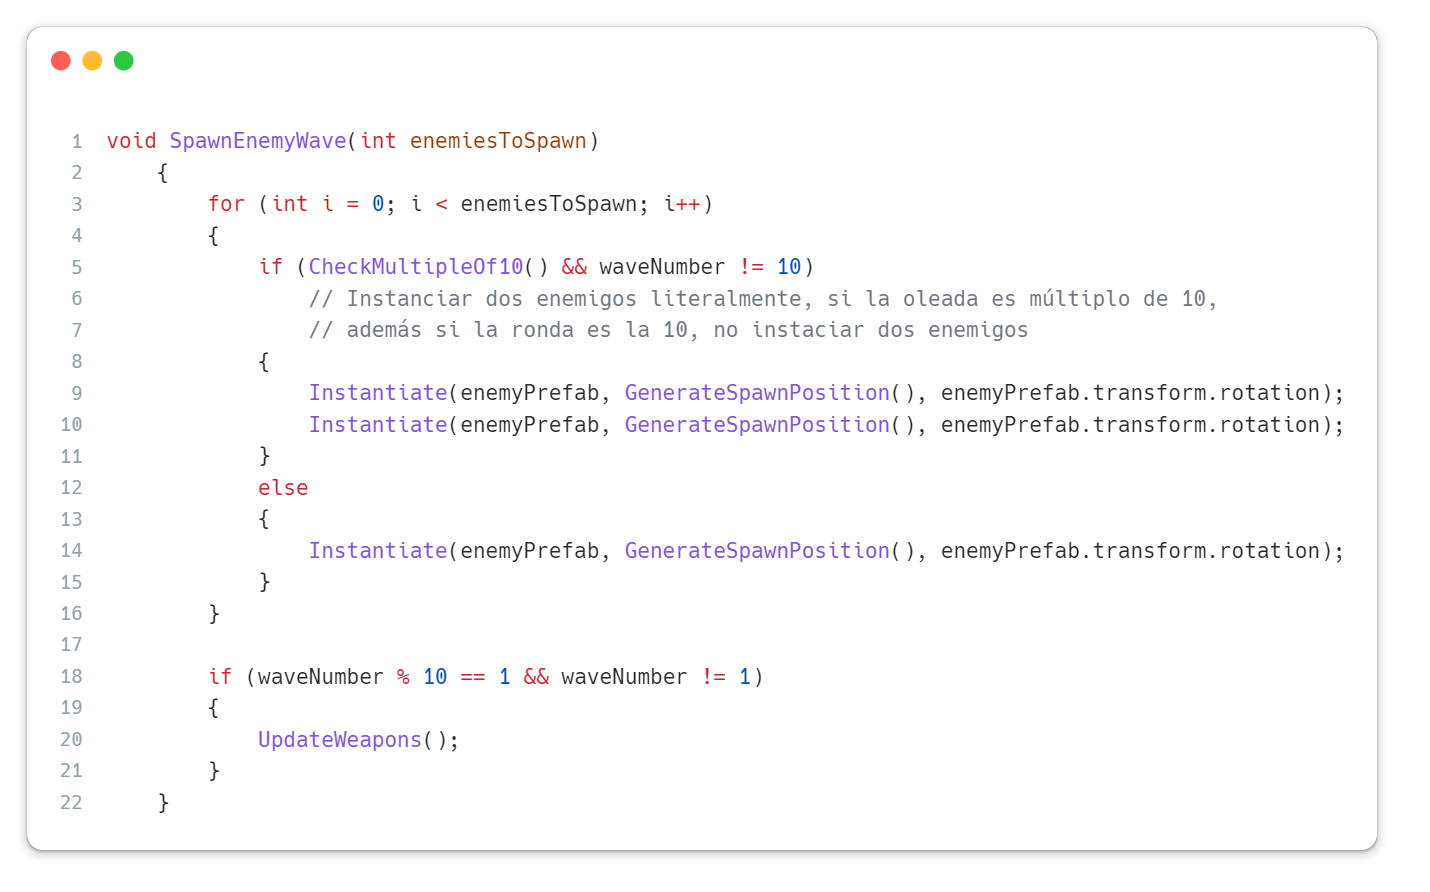
\includegraphics[width=\textwidth]{Images/Misc/SpawnEnemyWave.png}
                    \caption{Función para generar una oleada de enemigos}
                \end{figure}
                Esta función se encarga de generar la cantidad de enemigos que dicta según la ronda (cuyo número se gestiona con un parámetro de la función).\\

                Se inicializa un bucle que se repite según tantos enemigos se necesiten generar, haciendo una comprobación si la oleada es un múltiplo de 10, (es decir, que acabe en 0), genera dos enemigos; aunque para que el juego no sea muy injusto se ignora la ronda 10. \\

                Si no se cumple nada de esto solo se genera un enemigo.\\


            \newpage
            \subsubsection{Balas}
                \begin{figure}[H]
                    \centering
                    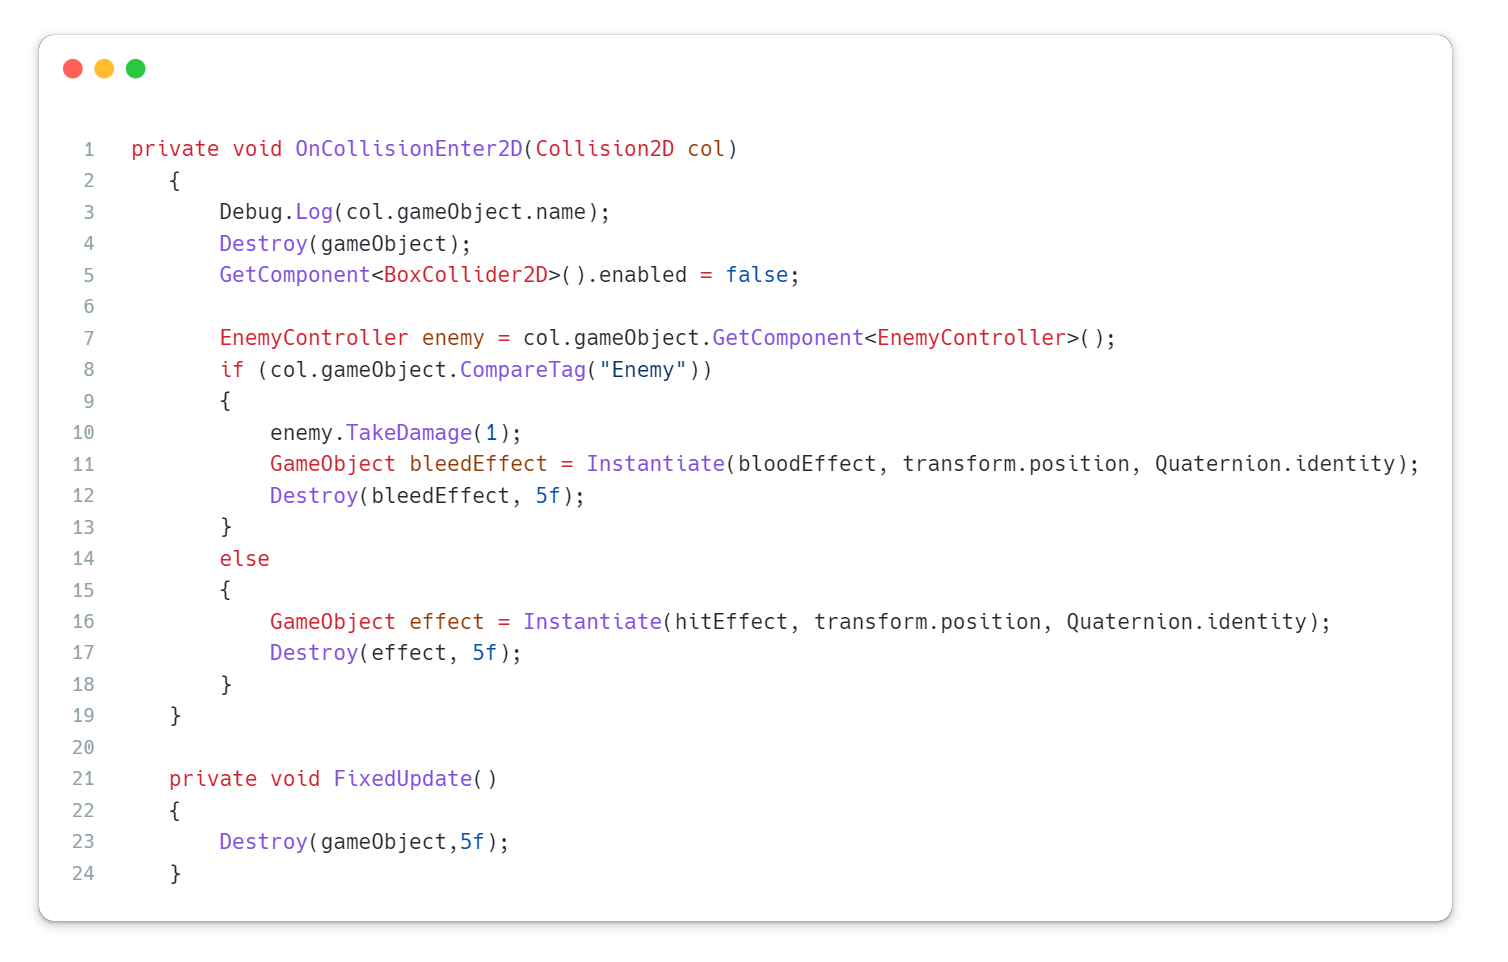
\includegraphics[width=\textwidth]{Images/Misc/bullet.png}
                    \caption{Script que contienen las balas}
                \end{figure}

                Para crear vínculos entre la bala y el objeto que colisiona se hizo que la bala gestionase esta colisión con el objeto.\\

                En primer lugar, justo antes del \textit{check} que comprueba con qué ha colisionado la bala, se comprueba si el objeto que ha colisionado es un enemigo, y si es así, se le resta vida al enemigo.\\
                
                Además, se instancia un sistema de partículas de sangrado adicional para reforzar el efecto de daño en el enemigo, explicado en el punto \ref{fig:enemigos}. \\

                Si no choca con nada (es decir, una pared) instancia otro efecto de partículas de impacto en la pared.\\

                Y para terminar, todos los efectos instanciados están en un temporizador (corrutina) que los destruye después de un tiempo.\\

            \newpage
            \subsubsection{Pivote de Arma}
                \begin{figure}[H]
                    \centering
                    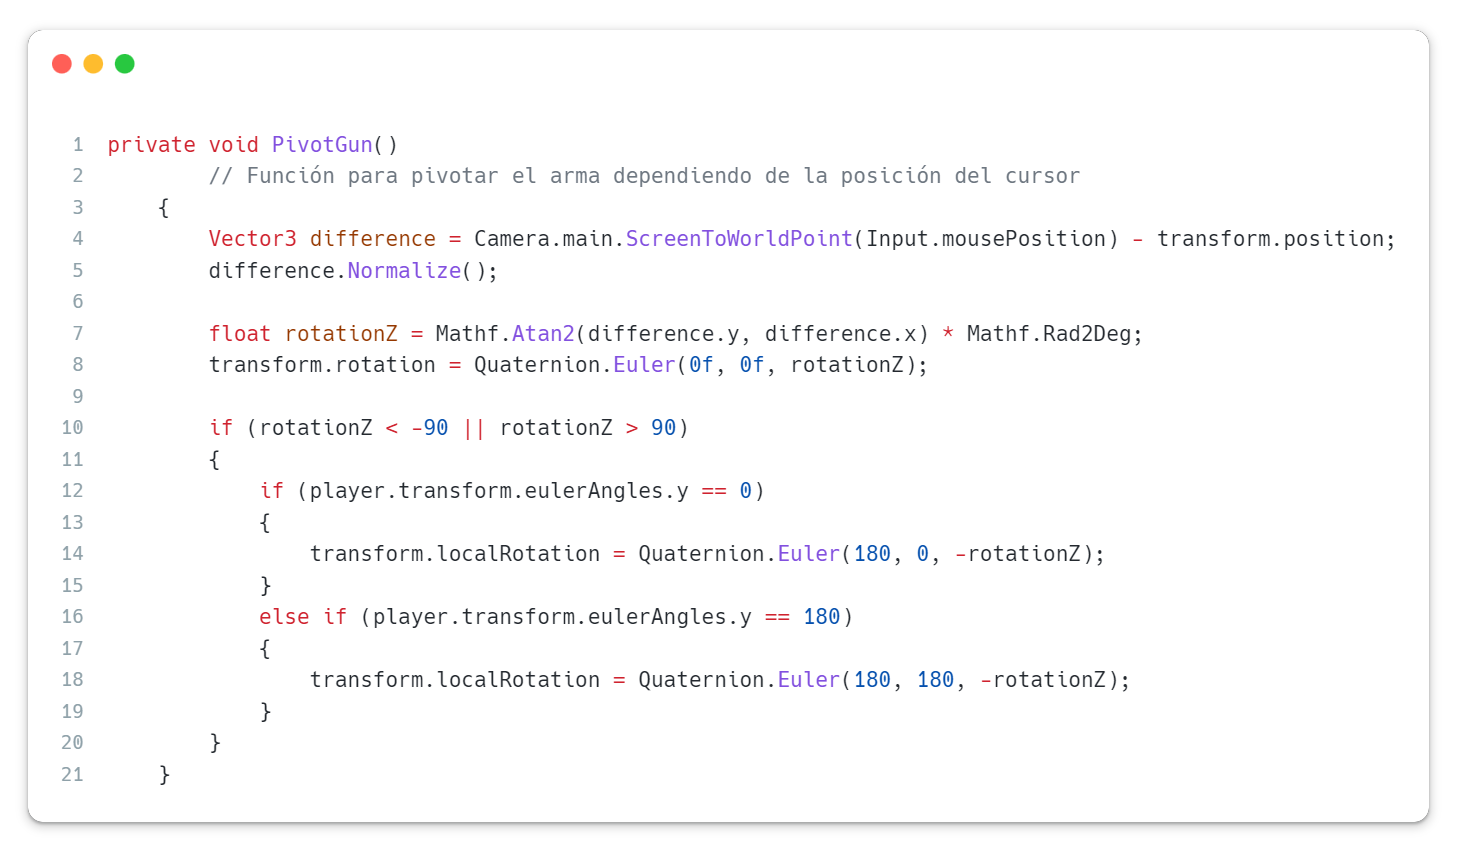
\includegraphics[width=\textwidth]{Images/Misc/pivot.png}
                    \caption{Script para pivotar el arma alrededor del personaje}
                \end{figure}

                Este script se encarga de pivotar el arma alrededor del personaje, para que el arma se vea en la posición correcta, tomando de referencia un \texttt{Vector3 difference} que es la resta del vector de la camara menos su componente \texttt{Transform}.\\

                Después, con \texttt{rotationZ} se crea una tangente con \texttt{Mathf.Atan2} con \texttt{difference} de Y e X; multiplicado por \texttt{Mathf.Rad2Deg} para convertir el resultado en grados sexagesimales. \\

                Con todo esto se crea una variable \texttt{transform.rotation} iguala a un \texttt{Quaternion.Euler} con \texttt{0} en X y Y y \texttt{rotationZ} en Z.\\

                Y por último, se crea una comparación para ver si la posición del cursor está a la derecha o a la izquierda del personaje.\\ 

                Si está a la derecha su rotación en Y es 0 y si está a la izquierda su rotación en Y es 180.\\

            \newpage
            \subsubsection{Gestor de Música}
            \begin{figure}[H]
                \centering
                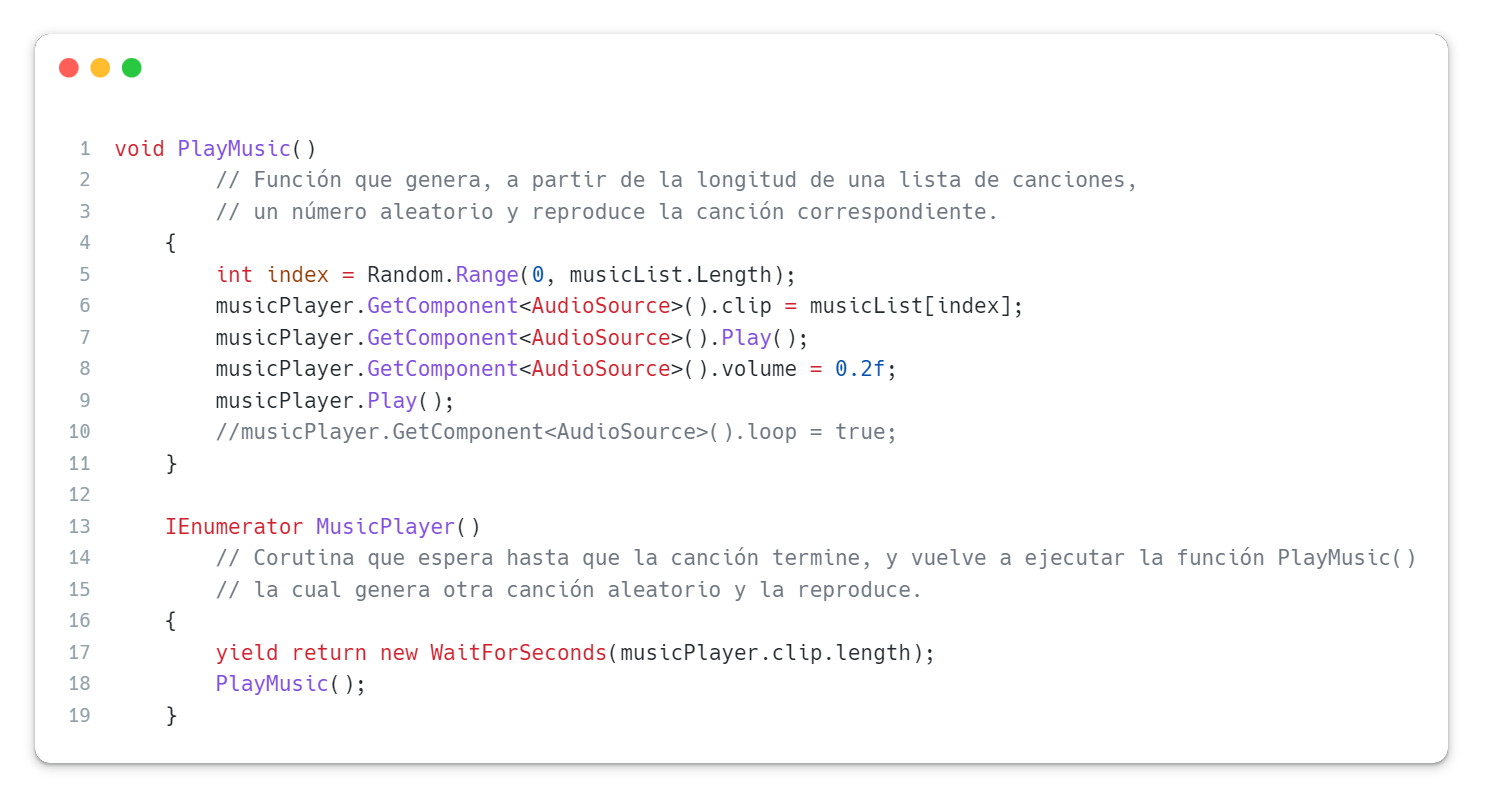
\includegraphics[width=0.7\textwidth]{Images/Misc/sound.png}
                \caption{Función para gestionar la música}
                \label{fig:musica}
            \end{figure}

            Esta función se encarga de gestionar la música del juego.\\
            En \texttt{void Awake()} se crea una lista de canciones, asignadas mediante el inspector:
            \begin{figure}[H]
                \centering
                \includegraphics[width=0.7\textwidth]{Images/Misc/inspectorsoundç.png}
                \caption{Lista de canciones}
            \end{figure}

            Para después en la función \texttt{PlayMusic()} escoger un índice aleatorio de la lista y reproducir la canción.\\
            Y para que pueda continuar la lista de canciones se usa una corrutina la cual se le asigna un \texttt{yield turn new WaitForSeconds} con la duración del clip de música. Así, cuando acabe la canción, se ejecutará la corrutina y se reproducirá la siguiente canción también de forma aleatoria.\\


\newpage
\section{Anexo}
    \subsection{Herramientas Utilizadas}
        \subsubsection{Programación y Creación de \textit{assets}}

            \begin{itemize}
                \item \textbf{Unity 2020.3}: \cite{Unity} para la creación del videojuego.
                \item \textbf{Unity Asset Store}: \cite{assetstore} para la búsqueda de \textit{assets}.            
                \item \textbf{Rider 2022.3}: \cite{rider} para la creación del código.
                \item \textbf{Itch.io}: \cite{itch} para la publicación del videojuego y obtención de \textit{assets}.
                \item \textbf{Aseprite}: \cite{aseprite} para la creación del logotipo del juego en pixel art.
            \end{itemize}
            
        \subsubsection{Documentación}

            \begin{itemize}                
                \item \textbf{De\textit{script}ion of the Assignment}: \cite{template} plantilla usada en este documento, con permiso CC BY 4.0.
                \item \textbf{VSCode}: \cite{vscode} para la creación del documento.
                \item \textbf{TinyTex}: \cite{tinytex} obtención de librerías, compilador y creador de documentos de \LaTeX
                \item \textbf{\LaTeX - Workshop}: \cite{workshop} extensión para convertir VSCode en un editor de \LaTeX completo.
                \item \textbf{LTeX}: \cite{ltex} revisión de ortografía y gramática del documento, así como limpieza del documento.
                \item \textbf{snappify}: \cite{seriouscode-gmbh-2022} para crear capturas de código con subrayado de funcions para el documento de \LaTeX.

                \item \textbf{Inter}: \cite{inter} fuente por defecto en el documento. 
                \item \textbf{Cascadia Code}: \cite{cascadia} fuente usada en fragmentos de código.

    \newpage
    \subsection{Licencia de plantilla}
        \textit{Nota del autor: Enlace a plantilla en bibliografía:~\ref{bibliografia}, cumpliendo con la licencia CC BY 4.0 de Creative Commons}\\
        \textit{Se han hecho los siguientes cambios:}
        \begin{figure}[H]
            \begin{itemize}
                \item Cambio de fuentes a \texttt{Inter} para la fuente por defecto y \texttt{Cascadia Code} para la fuente de código.
                Código de paquetería en preámbulo:
\begin{verbatim}
    \usepackage{inter}
    \usepackage{cascadia}
\end{verbatim}
                \item Logotipo en pie de página.
                \item Descripción de la asignación en encabezado de documento.
                \item Cambio de autor en el encabezado al principio del documento.
                \item Cambio de la portada: imagen, título y subtítulo.
                \item Adición de paquetería de \LaTeX adicional. 
            \end{itemize}
        \end{figure}
        \textit{Abstract: Template for de\textit{script}ion of assignment for master thesis topics at KU Leuven Ghent.}
        \end{itemize}
    \subsection{Referencias}
    
    \textbf{Videojuegos}
    \begin{itemize}
        \item Nuclear Throne \cite{vlaamber}
        \item Tormentor X Punisher \cite{E-Studio}
        \item Enter the Gungeon \cite{ETG}
        \item Hotline Miami \cite{dennaton}
    \end{itemize}

    \newpage
    \subsection{Bibliografía} \label{bibliografia}
        \printbibliography[heading = none]
        \nocite{*}

\end{document}